%\part{Variables Aleatorias}


\tableofcontents


\section{Variables aleatorias}

Supongamos que a cada punto del espacio muestral se le asigna un número.  Entonces hemos definido una \emph{función} en el espacio muestral  Esta función es llamada \emph{variable aleatoria} (o \emph{variable estocástica}) o de manera más precisa \emph{función aleatoria}. 


Usualmente, las variables aleatorias se denotan por letras mayúsculas como $X$ o $Y$. En general, una variable aleatoria tiene algún significado físico, geométrico, económico, financieros, etc.


[t]
\begin{exmp}
  \label{exmp:2.1}
Supongamos que una moneda se lanza dos veces de manera que el espacio muestral es $\set{HH,HT,TH,TT}.$  Digamos que $X$ representa el número de soles ($H$) que obtenemos.
\end{exmp}


\section{Funciones de probabilidad discretas}

 Sea $X$ una variable aleatoria discreta.  Supongamos que los valores que puede tomar son $x_{1},...,x_{k},$ arreglados en algún orden dado.  Supongamos también que esos valores
 tienen alguna probabilidad dada por
 \begin{align}
 \label{2.1}
 	P(X=x_{k})=f(x_{k}).
 \end{align}


{Función de probabilidad}
\begin{align}
\label{2.2}
P(X=x)=
\begin{cases}
f(x) & x=x_{k} \\
0	& \text{en otro caso}
\end{cases}
\end{align}



	En general, $f(x)$ será una función de probabilidad si
	\begin{align*}
		\begin{cases}
			f(x)\geq 0 \\
			\sum_{x}f(x)=1.
		\end{cases}
	\end{align*}



	\begin{exmp}
		\label{exmp:2.2}
		Encuentre la función de probabilidad correspondiente a la variable aleatoria $X$ del ejemplo \ref{exmp:2.1}.
	\end{exmp}



 \begin{exmp}
  \label{sol:2.1}
  Suponga que un par de dados se lanzan. Sea $X$ la variable aleatoria dada por la suma de los puntos. Encuentre la distribución de probabilidad de $X.$
 \end{exmp}



 \begin{exmp}
  \label{sol:2.2}
  Encuentre la distribución de probabilidad de niños y niñas en familias con 3 hijos, suponiendo la misma probabilidad para niños y niñas.
 \end{exmp}



\section{Funciones de distribución para variables aleatorias discretas}


	La función de distribución de una variable discreta $X$ se obtiene de la función de probabilidad a través de la siguiente fórmula
	\begin{align}
		\label{2.4}
		F(x) = P(X\leq x) = \sum_{u \leq x} f(u).
	\end{align}



	Si $X$ toma sólo un número finito de valores $x_{1},...,x_{n}$ entonces la función de distribución está dada por
	\begin{align}
		\label{2.5}
		F(x)=
		\begin{cases}
			0 & -\infty < x < 0 \\
			f(x_{1}) & x_{1} \leq x < x_{2} \\
			f(x_{1})+f(x_{2}) & x_{2} \leq x < x_{3} \\
			\vdots & \vdots \\
			f(x_{1})+\cdots+f(x_{n}) & x_{n} \leq x < \infty
		\end{cases}
	\end{align}



	\begin{exmp}
		\label{exmp:2.3}
		Encuentre la función de distribución para la variable aleatoria $X$ del ejemplo \ref{exmp:2.2} y obtenga su gráfica.
	\end{exmp}



	\begin{figure}
	\centering
	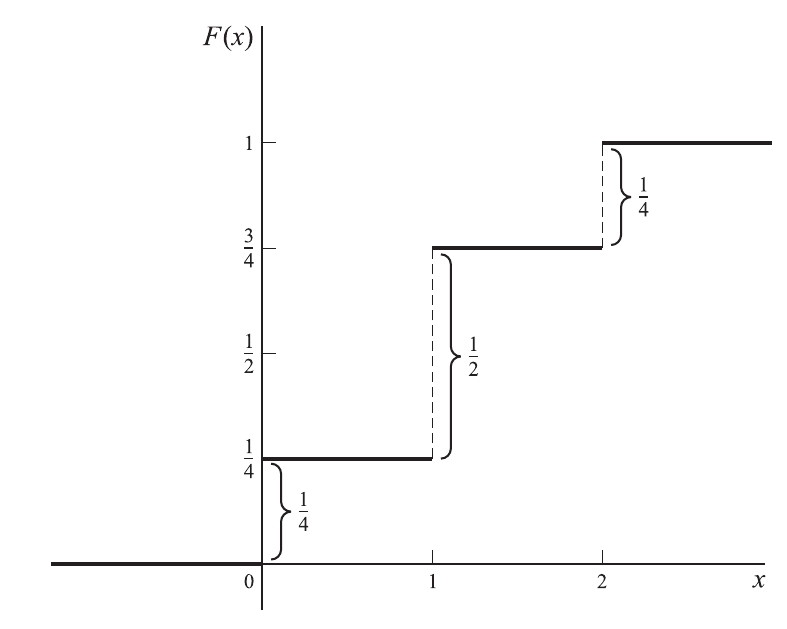
\includegraphics[height=7cm,keepaspectratio=true]{./pe/pands0201.png}
	% pands0201.png: 0x0 pixel, 300dpi, 0.00x0.00 cm, bb=
	\label{fig:0201}
\end{figure}



	\begin{rem}
		\begin{itemize}
			\item Los saltos en la función de distribución están determinados por el valor de la función de probabilidad. 
			\item Este tipo de funciones se conoce como \emph{función escalonada}.  Debe observarse que son \emph{continuas por la derecha.}
			\item La función de distribución es \emph{monótonamente creciente.}
		\end{itemize}

	\end{rem}



	La función de probabilidad se puede obtener a partir de la función de distribución con la siguiente fórmula
	\begin{align}
		\label{2.6}
		f(x)=F(x)-\lim_{u \to x^{-}}F(u).
	\end{align}



 \begin{exmp}
  \label{sol:2.3}
  \begin{enumerate}[(a)]
   \item Encuentre la función de distribución $F(x)$ para la variable aleatoria del problema resuelto \ref{sol:2.1};
   \item grafique esta función de distribución.
  \end{enumerate}

 \end{exmp}



 \begin{figure}[h]
 \centering
 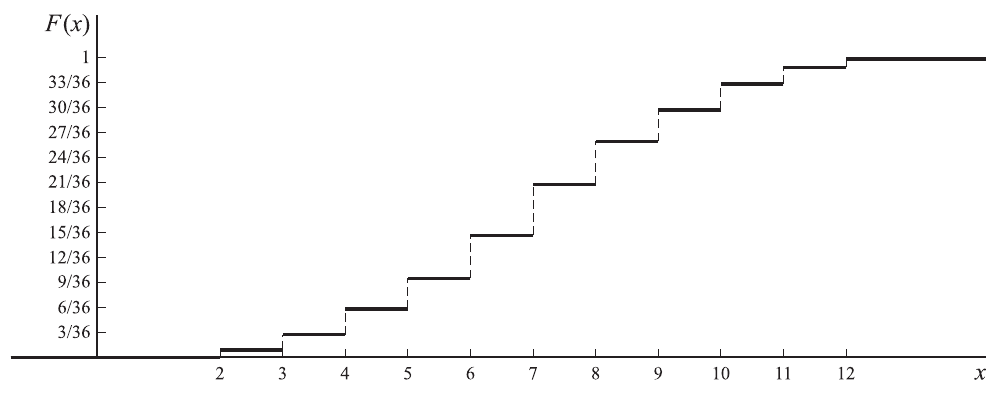
\includegraphics[width=10cm,keepaspectratio=true]{./pe/pands0206.png}
 % pands0206.png: 0x0 pixel, 300dpi, 0.00x0.00 cm, bb=
\end{figure}




 \begin{exmp}
  \label{sol:2.4}
  \begin{enumerate}[(a)]
   \item Encuentre la función de distribución $F(x)$ para la variable aleatoria del problema resuelto \ref{sol:2.2};
   \item grafique esta función de distribución.
  \end{enumerate}

 \end{exmp}



 \begin{figure}[h]
 \centering
 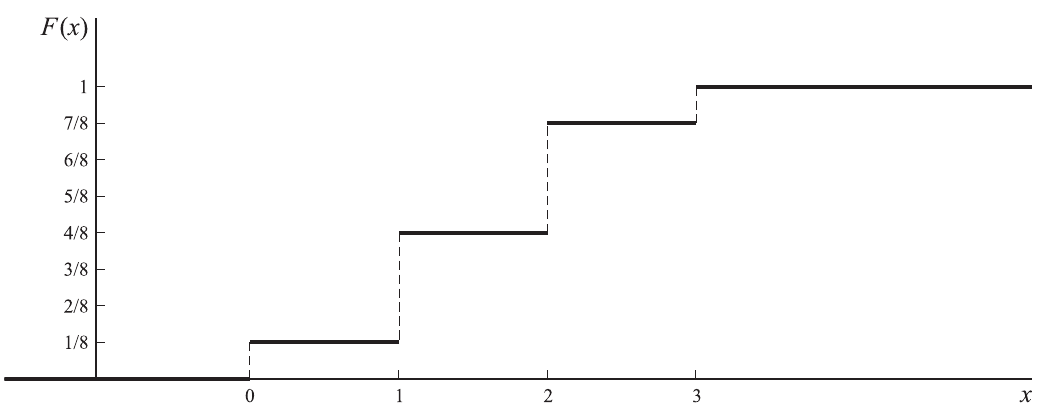
\includegraphics[width=10cm,keepaspectratio=true]{./pe/pands0207.png}
 % pands0206.png: 0x0 pixel, 300dpi, 0.00x0.00 cm, bb=
\end{figure}


\section{Variable Aleatorias Continuas}

	Una variable aleatoria no discreta $X$ se llama \emph{absolutamente continua} (o simplemente \emph{continua}) si su función de distribución puede ser representada como
	\begin{align}
		 \label{2.7}
		 F(x)=P(X \leq x)=\int_{-\infty}^{x} f(u)du, \; -\infty < x <\infty.
	\end{align}


	La función $f$ usualmente se llama \emph{densidad de probabilidad} y debe satisfacer las siguientes propiedades:
	\begin{enumerate}
		\item $f(x)\geq 0 $
		\item $\displaystyle \int_{-\infty}^{\infty}f(x)dx=1.$
	\end{enumerate}




	La probabilidad de que $X$ se encuentre entre dos valores $a$ y $b$ está dada por
	\begin{align}
		\label{2.8}
		P(a < x <b)=\int_{a}^{b}f(x)dx.
	\end{align}


[t]
	\begin{align}
		\label{exmp:2.4}
		P(X=a)=0.
	\end{align}


Por tanto, en \eqref{2.8} podemos reemplazar cualquier signo $<$ por $\leq.$

[t]
	\begin{exmp}
		\label{exmp:2.5}
		\begin{enumerate}[(a)]
			\item Encuentre la constante $c$ tal que la función
			\begin{align}
				f(x)=
				\begin{cases}
					cx^{2} & 0 < x < 3 \\
					0 & \texttt{en otro caso}
				\end{cases}
			\end{align}
			sea una función de probabilidad. 
			\item Calcule $P(1 < X < 2).$
		\end{enumerate}

	\end{exmp}


[t]
	\begin{exmp}
	  \label{exmp:2.6}
	  Encuentre la distribución de probabilidad para la variable aleatoria del ejemplo
	  \ref{exmp:2.5} y utilícela para calcular $P(1 < x \leq 2).$
	\end{exmp}



	La probabilidad de que $X$ se encuentre entre $x$ y $x+\Del x$ esta dada por
	\begin{align}
		\label{2.9}
		P(x \leq X \leq x+\Del x)= \int_{x}^{x+\Del x}f(u)du,
	\end{align} 
	de manera que si $\Del x \approx 0,$ tendremos que
	\begin{align}
		\label{2.10}
		P(x \leq X \leq x+\Del x)\approx f(x) \Del x.
	\end{align}



	También podemos deducir de \eqref{2.7}, al diferenciar de ambos lados, que
	\begin{align}
		\label{2.11}
		\dfrac{dF(x)}{dx} = f(x)
	\end{align}
en todos aquellos puntos en que $f(x)$ sea continua.  Es decir, la derivada de la función de distribución es la función de densidad.


	\begin{rem}
		Existen variables aleatorias que no son discretas ni continuas.  Por ejemplo
		\begin{align}
			F(x)=
			\begin{cases}
				0 & x <1 \\
				\frac{x}{2} & 1 \leq x < 2 \\
				1 & x \leq 2.
			\end{cases}
		\end{align}

	\end{rem}



 \begin{exmp}
  \label{sol:2.5} Una variable aleatoria $X$ tiene función de densidad
  \begin{align}
   f(x)=\dfrac{c}{x^{2}+1}, \; -\infty < x <\infty.
  \end{align}

  \begin{enumerate}[(a)]
   \item Encuentre el valor de $c$; 
   \item encuentre la probabilidad de que
   \begin{align*}
    \dfrac{1}{3}< X^{2} <1.
   \end{align*}

  \end{enumerate}

 \end{exmp}



 \begin{exmp}
  \label{sol:2.6}
  Encuentre la función de distribución correspondiente a la función de densidad del problema resuelto \ref{sol:2.5}
 \end{exmp}



 \begin{exmp}
  \label{sol:2.7}
  La función de distribución para una variable aleatoria $X$ es
  \begin{align}
   F(x)=
   \begin{cases}
    1-e^{-2x} & x\geq 0 \\
    0 & x <0
   \end{cases}
  \end{align}

  Encuentre
  \begin{enumerate}[(a)]
   \item la función de densidad;
   \item la probabilidad de que $X>2$;
   \item la probabilidad que $-3 < X \leq 4.$
  \end{enumerate}


 \end{exmp}



\section{Interpretación gráfica}


	La distribución $F(x)=P(X\leq x)$ es monótonamente creciente de $0$ a $1...$
	\begin{figure}[h]
	\centering
	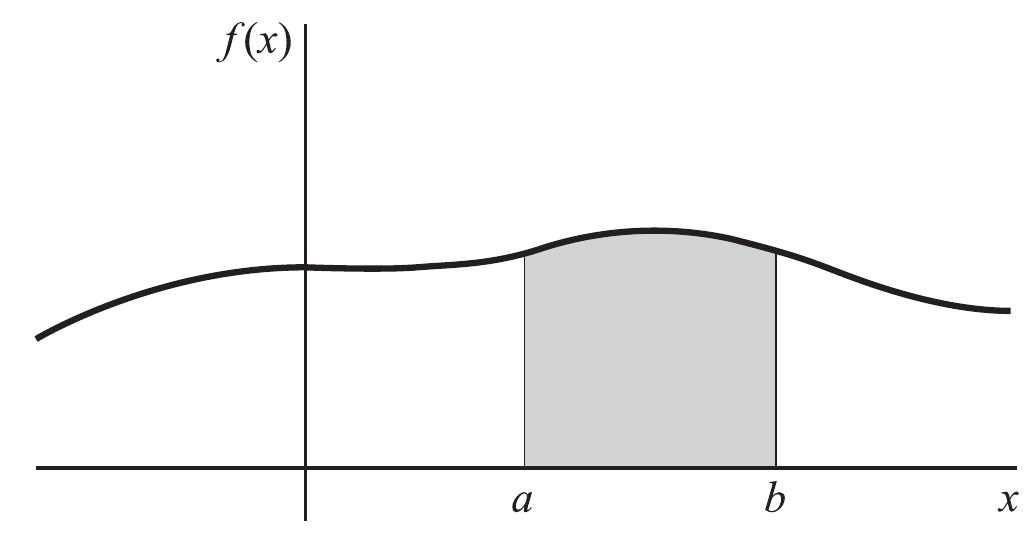
\includegraphics[height=5cm,keepaspectratio=true]{./pe/pands0202.png}
	% pands0202.png: 0x0 pixel, 300dpi, 0.00x0.00 cm, bb=
\end{figure}




  ...y el área bajo dicha curva es igual a $1.$
  \begin{figure}[h]
	\centering
	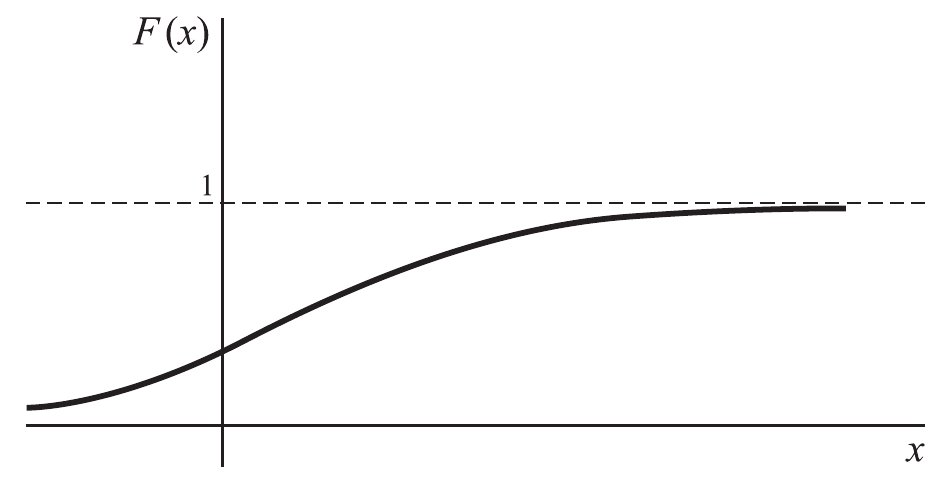
\includegraphics[height=5cm,keepaspectratio=true]{./pe/pands0203.png}
	% pands0203.png: 0x0 pixel, 300dpi, 0.00x0.00 cm, bb=
\end{figure}




\section{Distribución conjunta de probabilidad}


	Las ideas anteriores se generalizan fácilmente a dos o más variables.


{Caso discreto}
	Si $X$ y $Y$ son ambas variables aleatorias discretas, definimos la \emph{función de probabilidad conjunta} de $X$ y $Y$ por
	\begin{align}
	\label{2.13}
		P(X=x, Y=y)=f(x,y)
	\end{align}
 donde
\begin{enumerate}
	\item $f(x,y)\leq 0;$
	\item $\sum_{k}\sum_{y}f(x,y)=1.$
\end{enumerate}




	Supongamos que $X$ sólo toma uno de los $m$ valores $x_{1},...,x_{m},$ mientras que $Y$ tomas sólo toma uno de los $n$ valores $y_{1},...,y_{n}.$

	Entonces la probabilidad del evento $X=x_{j}, Y=y_{k}$ está dada por
	\begin{align}
	\label{2.14}
		P(X=x_{j}, Y=y_{k})=f(x_{j},y_{k})
	\end{align}



	Una función de probabilidad conjunta para $X$ y $Y$ puede ser representada por una \emph{tabla de probabilidad conjunta} como la siguiente:
	\begin{figure}[h]
	\centering
	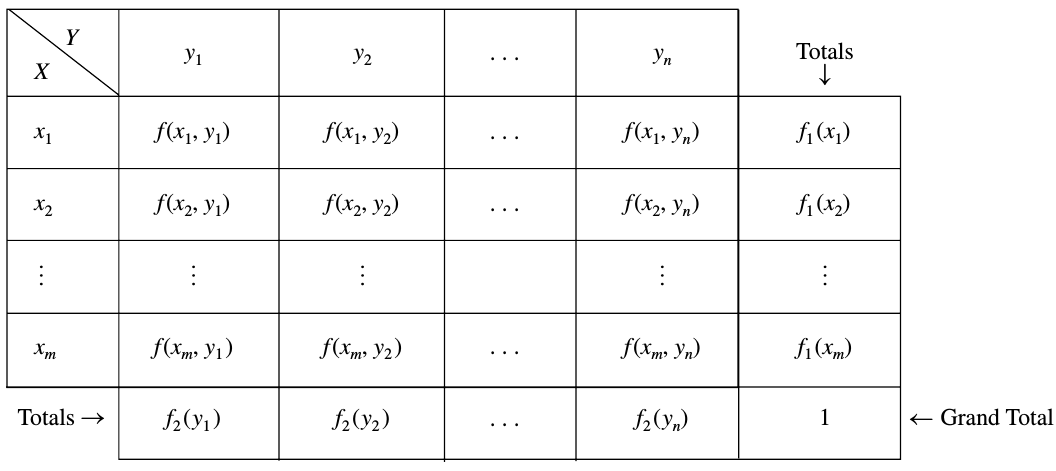
\includegraphics[height=5cm,keepaspectratio=true]{./pe/tab0203.png}
	% tab0203.png: 0x0 pixel, 300dpi, 0.00x0.00 cm, bb=
	\label{tab:0203}
\end{figure}



	La probabilidad de $X=x_{j}$ se obtiene de la siguiente manera
	\begin{align}
	\label{2.15}
		P(X=x_{j})=f_{X}(x_{j})=\sum_{k=1}^{n}f(x_{j},y_{k}).
	\end{align}



	De manera similar, la probabilidad de $Y=y_{k}$ se obtiene de la siguiente manera
	\begin{align}
	\label{2.16}
		P(Y=y_{k})=f_{Y}(y_{k})=\sum_{j=1}^{m}f(x_{j},y_{k}).
	\end{align}


 
 	Nos referiremos a $f_{X}(x)$ y $f_{Y}(y)$ como \emph{funciones de probabilidad marginal} de $X$ y $Y$ respectivamente.
 

	Observe que
	\begin{align}
	\label{2.17}
		\sum_{j=1}^{m}f_{X}(x_{j})=1,
		\sum_{k=1}^{n}f_{Y}(y_{k})=1,
	\end{align}
	lo cual se puede reescribir como
	\begin{align}
		\label{2.18}
		\sum_{j=1}^{m}\sum_{k=1}^{n}f(x_{j},y_{k})=1.
	\end{align}



	La \emph{función de distribución conjunta } está definida por
	\begin{align}
	\label{2.19}
		F(x,y)=P(X\leq x, Y\leq y)
		=\sum_{u\leq x}\sum_{v\leq y}f(u,v)
	\end{align}



{Caso continuo}
	El caso en el que ambas variables son continuas es obtenido de manera análoga reemplazando las sumas por integrales.


	La \emph{función de probabilidad conjunta} (o de manera más común \emph{función de densidad conjunta}) de $X$y $Y$ está definida por
	\begin{enumerate}
		\item $f(x,y)\geq 0;$
		\item $\displaystyle \int_{-\infty}^{\infty}\int_{-\infty}^{\infty}
		f(x,y) dxdy=1.$
	\end{enumerate}



	Gráficamente $z=f(x,y)$ representa una \emph{superficie de probabilidad}
\begin{figure}[h]
	\centering
	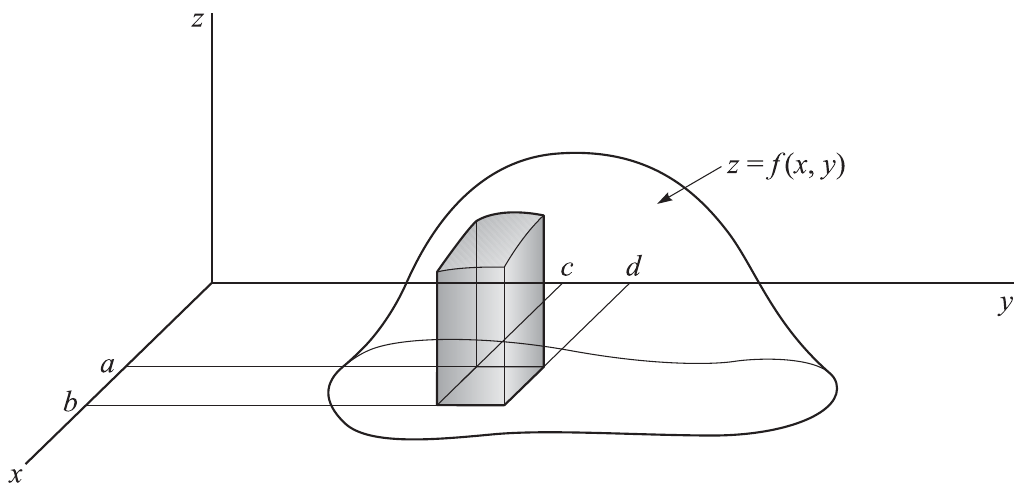
\includegraphics[height=3cm,keepaspectratio=true]{./pe/pands0204.png}
	% pands0204.png: 0x0 pixel, 300dpi, 0.00x0.00 cm, bb=
	\label{fig:2.4}
\end{figure}
tal que el volumen bajo la superficie es igual a $1.$


	\begin{align}
		\label{2.20}
		P(a<X<b,c<Y<d)=\int_{a}^{b}\int_{c}^{d}f(x,y)dydx.
	\end{align}



	A cada evento $A$ corresponde una región $\mathcal{R}_{A}$ del plano $xy$ tal que
	\begin{align}
	  \label{2.21}
		P(A)=\iint_{\mathcal{R}_{A}}f(x,y)dxdy.
	\end{align}



	La \emph{función de distribución conjunta} de $X$ y $Y$ en este caso está definida por
	\begin{align}
		\label{2.22}
	F(x,y)=P(X\leq x, Y\leq y)=
	\int_{-\infty}^{x} \int_{-\infty}^{y} f(u,v)dvdu.
	\end{align}



	Se sigue que
	\begin{align}
	 \dfrac{\partial^{2}F}{\partial x \partial y}=
	 f(x,y)  \label{2.23} \\
	  	 P(X\leq x)=F_{X}(x)=\int_{-\infty}^{x}\int_{-\infty}^{\infty} f(u,v)dvdu \label{2.24} \\
	 	 P(Y\leq y)=F_{Y}(y)=\int_{-\infty}^{\infty}\int_{-\infty}^{y} f(u,v)dvdu \label{2.25}
	\end{align}



 Diremos que $F_{X}(x),F_{Y}(y)$ son las \emph{funciones de distribución marginal,} o simplemente \emph{funciones distribuciones,} de $X$ y $Y$, respectivamente.


 Las derivadas de \eqref{2.24} y \eqref{2.25} con respecto a $x$ y $y$ son llamadas \emph{funciones de densidad marginal}, o simplemente las \emph{funciones de densidad,} de $X$ y $Y$ están dados por
 \begin{align}
 \label{2.26}
 \displaystyle
  f_{X}(x)=\int_{-\infty}^{\infty}f(x,v)dv, \;
  f_{Y}(x)=\int_{-\infty}^{\infty}f(u,y)du.
 \end{align}



\section{Variables Aleatorias Independientes}

 Supongamos que $X$ y $Y$ son variables aleatorias discretas.  Si los eventos $X=x$ y $Y=y$ son eventos independientes para todo $x,y,$  entonces diremos que $X,Y$ son v.a's independientes.


 En tal caso,
 \begin{align}
  \label{2.27}
  P(X=x,Y=y)=P(X=x)P(Y=y),
 \end{align}
o de manera equivalente
\begin{align}
 f(x,y)=f_{X}(x)f_{Y}(y).
\end{align}



 De manera inversa, si para todo $x,y$ la función de probabilidad conjunta $f(x,y)$ pueden ser expresada como el producto de funciones de probabilidad marginal $f_{X}(x)f_{Y}(y),$ entonces $X,Y$ son independientes.
 

 Si no pueden expresarse de dicha manera, entonces $X,Y$ son dependientes.


 Si $X,Y$ son v.a's continuas, diremos que son \emph{independientes} si los eventos $X\leq x$ y $Y\leq y$ son independientes para todo $x,y.$

 En tal caso, escribiremos
 \begin{align}
  \label{2.29}
  P(X\leq x, Y \leq y)=P(X\leq x)P(Y\leq y)
 \end{align} 
 o de manera equivalente
 \begin{align}
  F(x,y)=F_{X}(x)F_{Y}(y)
 \end{align}
 donde $F_{X}(x)$ y $F_{Y}(y)$ son las funciones de distribución marginal de $X,Y$ respectivamente.



 De manera inversa, si para todo $x,y$ la función de probabilidad conjunta $f(x,y)$ pueden ser expresada como el producto de funciones de probabilidad marginal $F_{X}(x)F_{Y}(y),$ entonces $X,Y$ son independientes.
 

 Si no pueden expresarse de dicha manera, entonces $X,Y$ son dependientes.


 Para v.a's independientes continuas, también es cierto que la función de densidad conjunta $f(x,y)$ es el producto de funciones $f_{X}(x)f_{Y}(y)$ y estas son las funciones de densidad marginal de $X,Y$ respectivamente.



 \begin{exmp}
  \label{sol:2.8}
  La función de probabilidad conjunta de dos variables discretas $X,Y$ está dada por
  \begin{align}
   f(x,y)=
   \begin{cases}
    c(2x+y) & 0\leq x \leq 2, \; 0 \leq y \leq 3 \\
    0 & \texttt{en otro caso}.
   \end{cases}
  \end{align}
  \begin{enumerate}[(a)]
   \item Encuentre el valor de la constante $c;$
   \item encuentre $P(X=2,Y=1);$
   \item encuentre $P(X\geq 1, Y\leq 2).$
  \end{enumerate}

 \end{exmp}



 \begin{figure}[h]
 \centering
 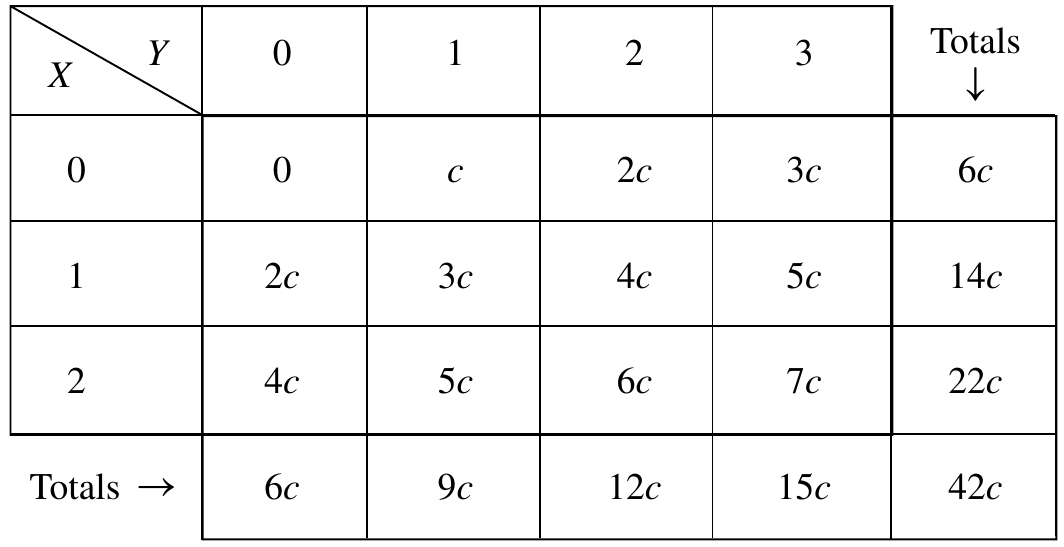
\includegraphics[width=10cm,keepaspectratio=true]{./pe/tab0206.png}
 % tab0206.png: 0x0 pixel, 300dpi, 0.00x0.00 cm, bb=
 \label{tab:2.6}
\end{figure}



 \begin{exmp}
  \label{sol:2.9}
  Encuentre las funciones de probabilidad marginal para $X$ y $Y$ en el problema resuelto \ref{sol:2.8}.
 \end{exmp}



 \begin{exmp}
  \label{sol:2.10}
  Muestre que las variables aleatorias del problema resuelto \ref{sol:2.8} son dependientes.
 \end{exmp}



 \begin{exmp}
  \label{sol:2.11}
  La función de densidad conjunta de dos variables aleatorias continuas $X$ y $Y$ es
  \begin{align}
   f(x,y)=
   \begin{cases}
    cxy & 0<x<4, \; 1<y<5\\
    0 & \texttt{en otro caso}.
   \end{cases}
  \end{align}

 \end{exmp}
\begin{enumerate}[(a)]
 \item Encuentre el valor de $c$;
 \item encuentre $P(1<X<2,2<Y<3)$;
 \item encuentre $P(X\geq 3, Y\leq 2)$.
\end{enumerate}



 \begin{exmp}
  \label{sol:2.12}
  Encuentre las funciones de probabilidad marginal de las v.a's $X,Y$ del problema resuelto \ref{sol:2.11}.
 \end{exmp}



 \begin{exmp}
  \label{sol:2.13}
  Encuentre la función de distribución conjunta para las v.a's del problema resuelto \ref{sol:2.11}.
 \end{exmp}



 \begin{center}
 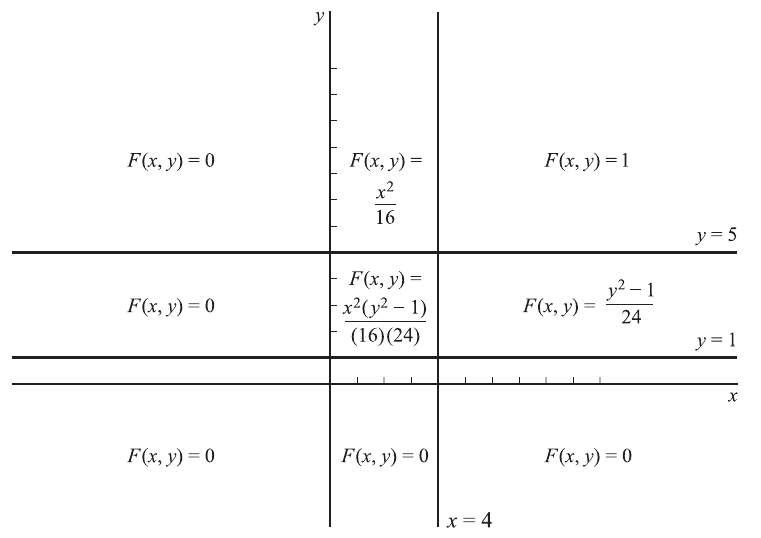
\includegraphics[width=10cm,keepaspectratio=true]{./pe/pands0209.png}
 % pands0209.png: 0x0 pixel, 300dpi, 0.00x0.00 cm, bb=
\end{center}




 \begin{exmp}
  \label{sol:2.14}
  En el problema resuelto \ref{sol:2.11}, encuentre $P(X+Y<3)$.
 \end{exmp}



 \begin{center}
 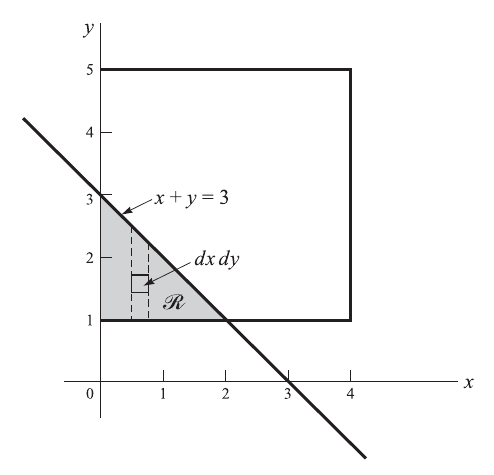
\includegraphics[height=8cm,keepaspectratio=true]{./pe/pands0210.png}
 % pands0210.png: 0x0 pixel, 300dpi, 0.00x0.00 cm, bb=
\end{center}



\section{Distribución Condicional}

 Nosotros ya sabemos que si $P(A)>0,$
 \begin{align}
  \label{2.41}
  P(B|A)=\dfrac{P(A\cap B)}{P(A)}.
 \end{align}



 Si $X,Y$ son v.a's discretas y tenemos los eventos $A=\set{X=x}, \; B=\set{Y=y},$ entonces \eqref{2.41} se convierte
 \begin{align}
  \label{2.42}
  P(Y=y|X=x)=
  \begin{cases}
   \dfrac{f(x,y)}{f_{X}(x)} & 0 < f_{X}(x)  \\
   0 & \texttt{en otro caso}
  \end{cases}
 \end{align}
 $f(x,y)=P(X=x,Y=y)$ es la función de probabilidad conjunta, mientras que $f_{X}(x)$ es la función de probabilidad marginal para $X.$


 Definimos la \emph{función de probabilidad condicional de $Y$ dado $X$} como
 \begin{align}
  \label{2.43}
  f(y|x)=
  \begin{cases}
   \dfrac{f(x,y)}{f_{X}(x)} & 0 < f_{X}(x)  \\
   0 & \texttt{en otro caso}
  \end{cases}
 \end{align}



 De manera similar, definimos la \emph{función de probabilidad condicional de $X$ dado $Y$} como
 \begin{align}
  \label{2.44}
  f(x|y)=
  \begin{cases}
   \dfrac{f(x,y)}{f_{Y}(y)} & 0 < f_{Y}(y)  \\
   0 & \texttt{en otro caso}
  \end{cases}
 \end{align}


 Estas ideas son fácilmente extensibles al caso donde $X,Y$ son v.a's continuas.


 Por ejemplo, la \emph{función de densidad condicional de $Y$ dado $X$} es
 \begin{align}
  \label{2.45}
  f(y|x)=
    \begin{cases}
   \dfrac{f(x,y)}{f_{X}(x)} & 0 < f_{X}(x)  \\
   0 & \texttt{en otro caso}
  \end{cases}
 \end{align}
 donde $f(x,y)$ es la función de densidad conjunta de $X$ y $Y$ y $f_{X}(x)$ es la función de densidad marginal de $X.$


 Usando \eqref{2.45} podemos por ejemplo encontrar que la probabilidad que $Y$  se encuentre entre $c$ y $d$ dado que $X=x$ es
 \begin{align}
  \label{2.46}P(c<Y<d|X=x)=
  \int_{c}^{d}f(y|x)dy.
 \end{align}




 \begin{exmp}
  \label{sol:2.27}
  Para la distribución del problema resuelto \ref{sol:2.8}, encuentre
  \begin{enumerate}[(a)]
   \item $f(y|2)$; y  
   \item $P(Y=1|X=2)$
  \end{enumerate}

 \end{exmp}



\begin{exmp}
 \label{sol:2.28}
  Si $X$ y $Y$ tienen función de densidad conjunta
 \begin{align}
  f(x,y)=
  \begin{cases}
   \frac{3}{4}+xy & 0<x<1, \; 0<y<1 \\
   0 & \texttt{en otro caso},
  \end{cases}
 \end{align}
encuentre
\begin{enumerate}[(a)]
 \item $f(y|x)$; 
 \item $P(Y>\frac{1}{2}| X = \frac{1}{2} )$.
\end{enumerate}

\end{exmp}



 \begin{exmp}
  \label{sol:2.29}
  La función de densidad conjunta de las variables aleatorias $X$ y $Y$ está dada por
  \begin{align}
   f(x,y)=
   \begin{cases}
    8xy & 0\leq x \leq 1, 0\leq y \leq x \\
    0 & \texttt{en otro caso}.
   \end{cases}
  \end{align}
Encuentre
\begin{enumerate}[(a)]
 \item la densidad marginal de $X$; 
 \item la densidad marginal de $Y$; 
 \item la densidad condicional de $X$; 
 \item la densidad condicional de $Y$.
\end{enumerate}

 \end{exmp}



 \begin{center}
 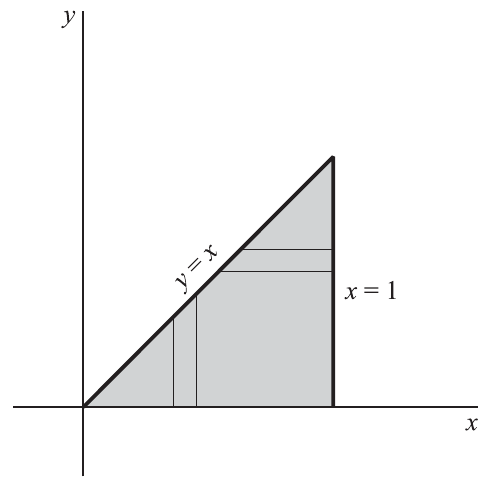
\includegraphics[height=7cm,keepaspectratio=true]{./pe/pands0217.png}
 % pands0217.png: 0x0 pixel, 300dpi, 0.00x0.00 cm, bb=
\end{center}



 \begin{exmp}
  \label{sol:2.30}
  Determine si las v.a's del problema resuelto \ref{sol:2.29} son independientes.
 \end{exmp}


